%This is the second chapter of the dissertation

%The following command starts your chapter. If you want different titles used in your ToC and at the top of the page throughout the chapter, you can specify those values here. Since Columbia doesn't want extra information in the headers and footers, the "Top of Page Title" value won't actually appear.

\pagestyle{cu}
\graphicspath{{./Chapter2/Figures/}}
\chapter[Liquid Xenon and Time Projection Chambers][Liquid Xenon and Time Projection Chambers]{Liquid Xenon and Time Projection Chambers}
\label{chap:liquid_xe}

Liquid xenon (LXe) direct detection experiments have dominated the sensitivity for WIMP masses $\gtrsim 20$ for approximately as
decade.  Even over liquid argon (LAr) the LXe results have been paved the way to new limits, surpassing on the way only those of other
LXe experiments.

Commercial business, such as steelmaking and coal gasification, rely relatively pure oxygen or nitrogen.  During the separation,
the small amount of xenon and krypton in the air is extracted into a mixture as a by-product.  A distillation process can uncouple
the two, leaving highly pure xenon.

%====================================
\section{General Properties}
\label{sec:properties}
Xenon has an atomic number of 54 with a mean mass of 131.293 g mol$^{-1}$.  Because it is a noble gas it does not easily undergo chemical
reactions with other elements.  It makes up 87 parts per billion (ppb) of the Earth's atmosphere at a density of
5.894 g L$^{-1}$.  \tabref{tab:xe_properties} gives some general chemical properties for xenon.

Xenon is the heaviest noble gas that is non-radioactive, with an atomic molar mass of $A = 131.293\ \mathrm{g\ mol^{-1}}$.  The naturally
occurring Xe isotopes are listed in
\tabref{tab:xe_isotopes}.  $^{136}Xe$, with a fractional percentage of 8.8573\%,
has been measured to undergo double beta decay with a half-life of $> 2.4 \times 10^{21}\ \mathrm{yrs}$ via
$2\nu \beta^{-} \beta^{-}$.  So while technically naturally occurring xenon is radioactive, the process is extremely rare.

Primary and secondary scintillation, which are the measured parameters in a time-projection chamber, occur when a particle interacts
with a Xe atom.  In the case of a neutron or neutrino scattering from the Xe nucleus a number of nuclear excitations are possible,
and are listed in \tabref{tab:xe_radioactive}.  The 39.6 and 80.2 keV lines from $^{129}$Xe and $^{131}$Xe are short-lived and typically
cannot be resolved from the scintillation of the scatter.  However, the 163.9 and 236.14 keV lines from $^{131\mathrm{m}}$Xe and
$^{129\mathrm{m}}$Xe are long-lived
enough to become uniformly distributed throughout the detector and can be used as a calibration source and measuring the electron
lifetime (\chapref{chap:purity}).

Xenon has several advantages that make it a good source for DM detection.  At \$2000 it is scaleable for larger detectors.  Its
large molar mass provides strong self-shielding, which reduces contamination in the region of interest due to external radiation
(discussed in \secref{}).  Furthermore, nearly 50\% of naturally occurring xenon is $^{129}$Xe or $^{131}$Xe, which gives it sensitivity to
spin-dependent interactions.  Its light and charge yields (\secref{}) are the highest among noble gases.  Finally, the amount of
intrinsic radioactivity comes only from trace amounts of radioactive noble gases that are present.

\begin{figure}
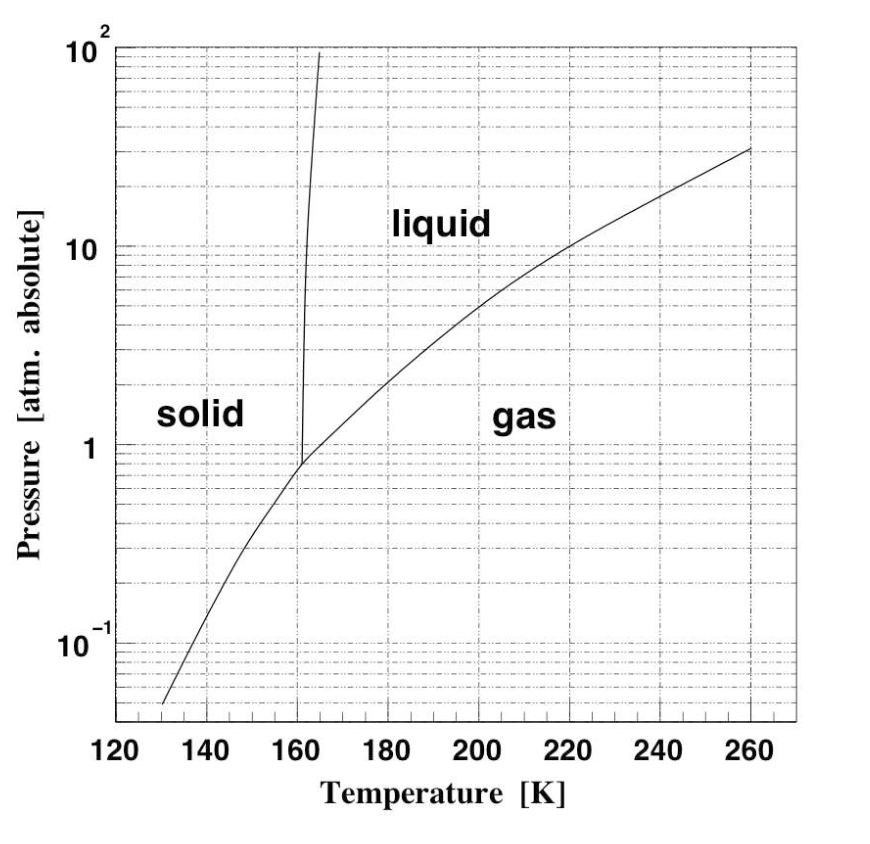
\includegraphics[width=0.6\textwidth]{PhaseDiagram}
\caption{Phase diagram of xenon(\citeref{Aprile2009})}
\label{fig:phase_diagram}
\end{figure}
 
\begin{table}[t]
 \centering
 \begin{tabular}{cc}
 \hline
 Chemical Property & Value \\
 \hline
 Atomic Number & 54 \\
 Molar mass & 131.293 g mol$^{-1}$ \\
 Melting point (1 atm) & -111.75 $^{\circ}$C \\
 Boiling point (1 atm) & -108.099 $^{\circ}$C \\
 Density as gas (0 $^{\circ}$C, 1 atm)  &  5.894 g L$^{-1}$ \\
 Density as liquid (-108.099 $^{\circ}$C, 1 atm) & 2.942 g cm$^{-3}$ \\
 Critical point & 16.59 $^{\circ}$C, 57.65 atm, 1.155 g cm$^{-3}$ \\
 Dielectric constant (liquid) & 1.95 \\
 Triple point & -111.74 $^{\circ}$C, 0.805 atm, 3.08 g cm$^{-3}$ \\
 Thermal conductivity & $5.65 \times 10^{-3}\ \mathrm{W\ m^{-1}\ K^{-1}}$ \\
 Covalent radius & $140 \pm 9$ pm \\
 \hline
 \end{tabular}
 \caption{Chemical properties for xenon}
\label{tab:xe_properties}
\end{table}


\begin{table}
 \centering
 \begin{tabular}{ccccc}
 \hline
 Isotope & Natural Abundance [\%] & Spin & Half-life & Decay mode \\
 \hline
 $^{124}$Xe & 0.0952 & 0 &  $> 1.6 \times 10^{14}\ \mathrm{yrs}$ & $2\nu \beta^{+} \beta^{+}$ \\
 $^{126}$Xe & 0.0890 & 0 & $> 4.7-12 \times 10^{25}\ \mathrm{yrs}$ & $2\nu \beta^{-} \beta^{-}$ \\
 $^{128}$Xe & 1.9102 & 0 & stable & - \\
 $^{129}$Xe & 26.4006 & 1/2 & stable & - \\
 $^{130}$Xe & 4.0710 & 0 & stable & - \\
 $^{131}$Xe & 21.232 & 3/2 & stable & - \\
 $^{132}$Xe & 26.9086 & 0 & stable & - \\
 $^{134}$Xe & 10.4357 & 0 &  $> 5.8 \times 10^{22}\ \mathrm{yrs}$ & $2\nu \beta^{-} \beta^{-}$ \\
 $^{136}$Xe & 8.8573 & 0 &  $> 2.4 \times 10^{21}\ \mathrm{yrs}$ & $2\nu \beta^{-} \beta^{-}$ \\
 \hline
 \end{tabular}
 \caption{Properties of naturally occurring Xe isotopes.  Decays of \ce{^{124}Xe}, \ce{^{126}Xe}, and \ce{^{134}Xe} have not been observed
 but are predicted.  Half-life and decay information is taken from \citeref{Singh2007, Barros2014}.}
\label{tab:xe_isotopes}
\end{table}


\begin{table}
 \centering
 \begin{tabular}{ccc}
 \hline
 Isotope & Energy [keV] & Half-life \\
 \hline
 \ce{^{129}Xe} & 39.6 & 0.97 ns \\
 \ce{^{129m}Xe} & 236.1 & 8.88 d \\
 \ce{^{131}Xe} & 80.2 & 0.48 ns \\
 \ce{^{131m}Xe} & 163.9 & 11.93 d \\
 \hline
 \end{tabular}
 \caption{Nuclear excited states for naturally occurring xenon in the energy range direct DM searches are sensitive too.}
 \label{tab:xe_radioactive}
\end{table}

\begin{figure}
\centering
\includegraphics[width=0.8\textwidth]{Figure 1 from SeeFig15}
\end{figure}



%====================================
\section{Signal Production}
\label{sec:scintillation}
Radiation scattering off a xenon atom will produce a prompt or primary scintillation as a result of electronic excitation or recombination
from ionized electrons that emit photons as they de-excite.  Secondary scintillation results from ionized
electrons that do not recombine and is measured only in a time-projection
chamber (TPC).  In this section
and the remainder of the chapter I will consider interactions in xenon in the presence of an electric field, unless otherwise
specified.



%========
\subsection{Primary Scintillation}
\label{subsec:primary}
When a particle scatters off a Xe atom it can excited or ionize its valence electrons.  Here we refer to excited atoms Xe$^{*}$ as
excitons.  An ionized electron can then escape or recombine with the Xe$^{+}$.  Excitons can form with another Xe atom to create
dimers, Xe$_{2}^{*}$, commonly referred to as excimers.  The processes recombination is shown in \eqnref{eq:recomb}, where $Q$
represents heat.  It should be stated that the $e^{-}$ in the recombination process is from the same or another ionized atom.  If
no electric field is , so the primary scintillation will not reflect the true

If
an electric field is applied some $e^{-}$ will be forced away from the interaction, thereby lowering recombination and the primary
scintillation.  This effect depends on the strength of the electric field.  However, even if no field is applied there will not be
100\% recombination as some of the freed $e^{-}$ will escape the electromagnetic pull.

\begin{equation}
\mathrm{Xe}^{+} + \mathrm{Xe} \rightarrow \mathrm{Xe}_{2}^{+} \\
\mathrm{Xe}_{2}^{+} + e^{-} \rightarrow \mathrm{Xe}^{**} + \mathrm{Xe} \\
\mathrm{Xe}^{**} \rightarrow \mathrm{Xe}^{*} + Q \\
\label{eq:recomb}
\end{equation}

\noindent At this point the Xe$^{*}$ that has been born of the ionization and recombination process is equivalent to one from simply the
excitation.  At this point they must de-excited via \eqref{eq:deexcite}.  Xe$_{2}^{*}$ is in either a singlet
($^{1}\Sigma$) or triplet ($^{3}\Sigma$) state, and de-excites to the ground state.

\begin{equation}
\mathrm{Xe}^{*} + \mathrm{Xe} \rightarrow \mathrm{Xe}_{2}^{*} \\
\mathrm{Xe}_{2}^{*} \rightarrow 2\mathrm{Xe} + \gamma
\label{eq:deexcite}
\end{equation}

\noindent $\gamma$ is the average de-excitation energy that carries a wavelength of 178 nm.  The lifetimes for the singlet and triplet
excimers are $3.1 \pm 0.7$ ns and $24 \pm 1$ ns, respectively (\citeref{Mock2014}).  The single-to-triplet ratios for
various interaction types are shown in \tabref{tab:singlet_to_triplet}.  An important method for detecting WIMPS is ER-NR
discrimination, and we see that NR recoils result in a substantially higher fraction of singlet states.  Unfortunately the lifetimes
are too short to resolve in a TPC to be able to use for discrimination.  This makes single-phase LXe detectors
less desirable than liquid argon (LAr), which has single and triplet states of $< 6.2$ ns and $1.30 \pm 0.06\ \mathrm{\mu s}$
(\citeref{Heindl2011}).

\begin{table}[t]
 \centering
 \begin{tabular}{cc}
 \hline
 Event & Single/Triplet Ratio \\
 \hline
 ER (direct excitation from $\gamma$) & $0.17 \pm 0.05$ \\
 ER (recombination from $\gamma$) & $0.8 \pm 0.2$ \\
 ER (from $\alpha$) & $2.3 \pm 0.51$ \\
 NR (from neutron) & $7.8 \pm 1.5$ \\
 \hline
 \end{tabular}
 \caption{Error-weighted average of world data for single/triplet ratio for various scattering cases (\citeref{Mock2014}).}
\label{tab:singlet_to_triplet}
\end{table}

\eqnref{eq:recomb} and \eqnref{eq:deexcite}
depict the entire microphysical processes for $\beta$ and $\gamma$ interactions (\citeref{Hitachi2005}).  However, in nuclear recoils
it has been observed that two excitons may collide and free an electron as shown in \eqnref{eq:biexcitonic}.




%========
\subsection{Secondary Scintillation}
\label{subsec:secondary}
In an electric field $E$ an \electron that is freed but does not recombine with its parent or other ionized atoms will move anti-parallel
to the field at drift velocity $v_{d}$.  At fields of $\lesssim 100\ \mathrm{V\ cm^{-1}}$ drift velocity is nearly proportional to
$E$ and is given by $v_{d} = \mu E$
where $\mu$ is the electron mobility.  For this energy region $\mu \sim 2200\ \mathrm{cm^{2}\ V^{-2}\ s^{-1}}$ (\citeref{Yoo2015}).  As
$E$ increases $v_{d} \propto E^{1/2}$ and ultimately flattens at $\sim 3\ \mathrm{mm\ \mu s}$.  \figref{fig:drift_velocity} shows \vd
as a function of $E$ and \tabref{tab:drift_velocity} gives the approximate relationship.

The strength of $E$ affects the number of electrons freed, as a larger field decreases
recombination electron-ion recombination.  In liquid noble gas detectors used for DM searches such a field can be used to drift the
\electron to the surface of the liquid, where they are extracted across a small region of gas.  Doing so will produce secondary
scintillation as the \electron will energize the atoms in the gas, freeing more \electron in turn.  Because the amount of scintillation
produced per electron is independent of the number of electrons extracted this is also known as proportional scintillation.  Thus, by
measuring this scintillation the number of \electron extracted can be determined.  Details of \electron drift and proportional
scintillation is found in \secref{subsec:tpcs_working_principle}.

For $E \lesssim 100\ \mathrm{V\ cm^{-1}}$ \vd$\propto E$, $100 \lesssim E \lesssim 10^{3-4}$
\vd$\propto E^{1/2}$, and $E \gtrsim 10^{4}$ \vd plateaus at $\sim 3\ \mathrm{mm\ \mu s^{-1}}$ (\citeref{Miller1968}).

\begin{table}
 \centering
 \begin{tabular}{cc}
 \hline
 $E$ [V cm$^{-1}$] & \vd [mm $\mu$s$^{-1}$] \\
 \hline
 $\lesssim 100$ & \vd$\propto E$ \\
 $\sim 100-10^{3-4}$ & \vd$\propto E^{1/2}$ \\
 $\gtrsim 10^{4}$ & \vd$\sim 3$ \\
 \hline
 \caption{Drift velocity \vd as a function of electric field $E$ for LXe}
 \end{tabular}
 \label{tab:drift_velocity}
\end{table}

\begin{figure}
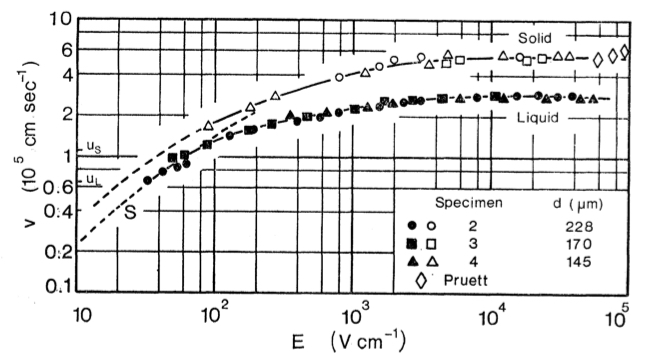
\includegraphics[angle=0.5, width=0.8\textwidth]{DriftVelocity}
\caption{Drift velocity for solid and liquid xenon}
\label{fig:drift_velocity}
\end{figure}




%====================================
\subsection{Stopping Power}
\label{subsec:stopping_power}
The track structure is defined by the distribution of \electron, ions, and excitons when all \electron have slowed to sub-excitation
speed (\citeref{Chepel2013}).  This has a major role in determining the subsequent response of atoms and \electron.  Track structures
vary considerably with respect to different particles and linear energy transfer (LET).  Still, tracks typically have a cylindrical
structure with secondary branches resulting from $\delta$-rays.

A particle that loses energy through inelastic collisions with electrons (prompting excitation and ionization) will produce an electronic
recoil.  The energy lost per unit
length is the electronic stopping power $dE/dx$.  It is related to the LET and depends on the
type and energy of the particle and properties of the
medium, including density and composition.  A larger electronic stopping power indicates the particle will slow more quickly, thereby
depositing its energy more densely along its track.

The energy density affects recombination between \electron and ions and is discussed in \secref{subsec:recombination}.  Xenon
has a large stopping power - in part to its large atomic mass - that slows particles relatively efficiently.  One benefit of this
is self-shielding, which protects the interior of the detector from outside radiation.  Higher self-shielding restrains external
radiation from penetrating deep into the detector,
allowing a larger fiducial volume (FV) for dark matter searches.  Because the stopping power is proportional to the
density of the medium, LXe is more effective at self-shielding than liquid argon ($1.395\ \mathrm{g\ cm^{-3}}$) and liquid neon
($1.207\ \mathrm{g\ cm^{-3}}$).

By dividing the stopping power by the medium's density we get a function that is mainly a function of the radiating particle known as
the mass stopping power.  This is shown for $\alpha$, $e^{-}$, and protons in \figref{fig:mass_stopping_power}.  We see that for the DM
region of interest ($1-100$ keV) as \electron
energy increases the stopping power decreases, while for $\alpha$ and protons the reverse is true.  Multiplying by the density of LXe
$\rho_{\mathrm{LXe}}$ gives an electron stopping power of $0.65-30\ \mathrm{keV\ \mu m^{-1}}$ for \electron and
$\sim 20-900\ \mathrm{keV\ \mu m^{-1}}$ for $\alpha$ and protons.

We can see that in
the dark matter search region ($1-100$ keV) $e^{-}$ decrease by a factor of $\sim 10$.  Multiplying by the density of LXe we get the
electronic stopping power to be $\sim 0.65-30\ \mathrm{keV\ \mu m^{-1}}$.  \alphadecays are typically $> 5.5$ MeV and thus have a stopping
power of $\sim 600-2000\ \mathrm{keV\ \mu m^{-1}}$.  We see that particle tracks are $\mathcal{O}(10)\ \mathrm{\mu m}$, so particles
that originate at or outside the surface of the detector will never make it into the FV with any reasonable probability.

\begin{figure}[t]
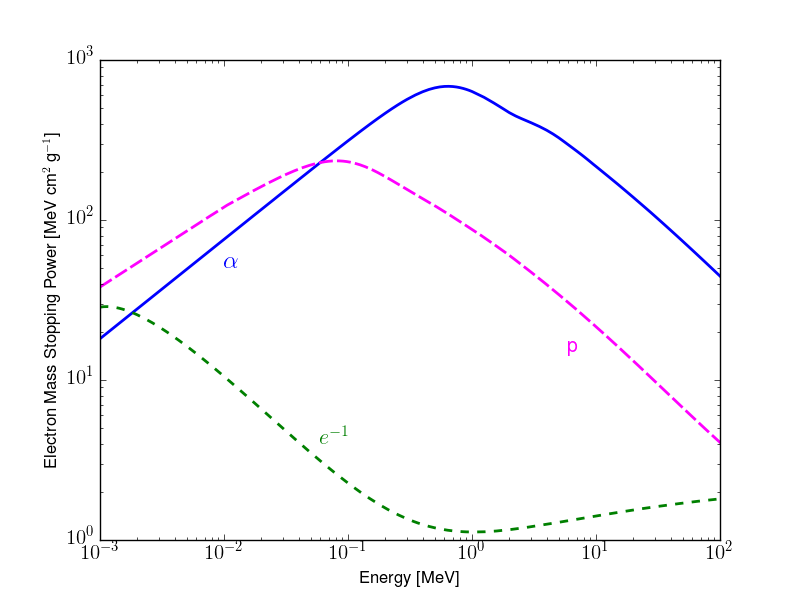
\includegraphics[width=0.8\textwidth]{MassStoppingPower}
\caption{Electron mass stopping power for $\alpha$, $e^{-}$, and protons.  (\citeref{Berger2018a})}
\label{fig:mass_stopping_power}
\end{figure}

Since a higher stopping power translates to a larger decrease in energy, there will be a higher ionization density in the particle
track.  This has implications that will be discussed in \secref{}.

For particles that induce a nuclear recoil we must also consider the nuclear stopping power, which is the energy lost per unit length from
atomic collisions that transfer kinetic energy to the nucleus.  Thus for NR the total stopping power is

\begin{equation}
\bigg( \frac{dE}{dx} \bigg)_{\mathrm{tot}} = \bigg( \frac{dE}{dx} \bigg)_{\mathrm{elec}} + \bigg( \frac{dE}{dx} \bigg)_{\mathrm{nuc}}
\end{equation}



%========
\subsection{Recombination}
\label{subsec:recombination}
An essential ingredient to understanding the particle interaction and energy is recombination.  It is related to ionization density,
thermal energy of ionized atoms and \electron, electron mobility, diffusion rate, electric field, probability of recombination when
and \electron meets an ion, and more.

An earlier theory by Onsager addressed this by defining what is known
as the Onsager radius, or the distance between parent
ion and \electron where the Coulomb energy equals the \electron thermal energy (\citeref{Onsager1938}).  An \electron within this
radius will be unlikely to
escape so will recombine with its parent (the probability of escape at the Onsager radius is e$^{-1}$).  On the contrary, an \electron
with $E_{\mathrm{thermal}} > E_{\mathrm{Coulomb}}$ will escape - even without the presence of an Electric field.  This results in a decrease of expected
photons.  It is expected in the absence of a field recombination may occur on timescales $> 1$ ms but this is much larger than the
observation window.  The thermalization range for LXe is $4000-5000$ nm, far higher than the Onsager radius of $49$ nm
(\citeref{Doke2002}).

A shortcoming of the Onsager radius is that it treats the interactions between Xe$^{+}$ and \electron as strictly Coulomb.  However,
the high coefficient of polarization of LXe produces dipole moments in the ions, causing the electric field to fall faster than
$1/r$.  In fact, the potential is steep enough that the ion travels via phonon-assisted tunneling (\citeref{Thomas1987}), forcing its
mobility to be significantly smaller than that of the electrons.

As a result of these inconsistencies another model was proposed that used diffusion but with a term that represents the rate of
recombination depends on
the density of \electron and ions independently, first proposed in \citeref{Jaffe1913}.  It is derived by considering

\begin{equation}
\frac{\partial N_{+}}{\partial t} = -u_{+} \mathbf{E} \cdot \nabla N_{+} + d_{+} \nabla^{2} N_{+} - \alpha N_{+} N_{-}
\label{eq:diff_plus}
\end{equation}

\begin{equation}
\frac{\partial N_{-}}{\partial t} = u_{-} \mathbf{E} \cdot \nabla N_{-} + d_{-} \nabla^{2} N_{+} - \alpha N_{+} N_{-}
\label{eq:diff_minus}
\end{equation}

\noindent where $N_{\pm}$ are the ion ($+$) or electron ($-$) charge distributions, $\mu_{\pm}$ are the electron mobilities, $d_{\pm}$
and $\alpha$
are the coefficients for diffusion and recombination, and $\mathbf{E}$ is the electric field.  The terms on the right sides of
\eqref{eq:diff_plus} and \eqref{eq:diff_minus} correspond to the drift, diffusion, and recombination, going from left to right.  The
diffusion in xenon is small and can be ignored.  Likewise the ion mobility $\mu_{+}$ is several orders of magnitude smaller than that
of the electron and is disregarded.  Thus \eqref{eq:diff_plus} and \eqref{eq:diff_minus} can be simplified to

\begin{equation}
\frac{\partial N_{+}}{\partial t} = - \alpha N_{+} N_{-}
\label{eq:diff_simple_plus}
\end{equation}

\begin{equation}
\frac{\partial N_{-}}{\partial t} = u_{-} E \frac{\partial d_{-}}{\partial z} - \alpha N_{+} N_{-}
\label{eq:diff_simple_minus}
\end{equation}

\noindent which can be solved exactly.  After some integration and algebra, which is not shown here but is detailed in
\citeref{Thomas1987}, the recombination fraction can be solved as

\begin{equation}
r = 1 - \frac{1}{\xi} \mathrm{ln}(1 + \xi),\ \ \xi = \frac{N_{i} \alpha}{4 a^{2} u_{-} E}
\label{eq:ti_recomb}
\end{equation}

\noindent where a box of dimension $a$ contains charge quantity $N_{i}$ uniformly spread.  This is known as the Thomas-Imel box model,
and has been successful at explaining recombination measurements as shown in \figref{fig:ti_recomb}.  Zero recombination corresponds to
$\xi \rightarrow 0$ and total is given by $\xi \rightarrow \infty$.  Note that $E = 0$ equates to total recombination, though as
mentioned above, this may occur outside of the typical observation window.

\begin{figure}
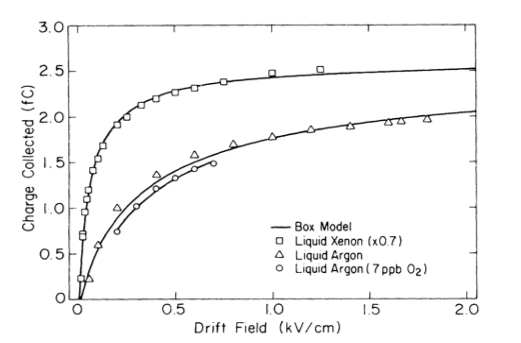
\includegraphics[width=0.8\textwidth]{TIRecombination}
\caption{Measurements of charge collected $q \propto 1 - r$ for LAr and LXe vs. $E$.  Squares correspond to LXe and were measured with
$\xi E = 0.15\ \mathrm{kV\ cm^{-1}}$.  Triangles and circles are LAr and were measured at $\xi E = 0.84\ \mathrm{kV\ cm^{-1}}$.  Curves
are best fit for box model (\citeref{Thomas1987}).}
\label{fig:ti_recomb}
\end{figure}

The Thomas-Imel box model works well for short particle tracks but does not accurately predict long.  At longer particle tracks a Birks'
Law (originally developed for foro organic scintillators, \citeref{Birks1964}) derivation for liquid noble gases yields

\begin{equation}
\frac{dN_{\pm}}{dt} = -\alpha N_{+} N_{-}
\label{eq:birks_diff}
\end{equation}

\noindent for volume recombination - that is, for \electron to recombine with an ion other than their parent.  Here $N_{\pm}$ and
$\alpha$ have the same definitions as in the Thomas-Imel model.  Simplification is used to equate the number of ions to electrons
$N_{+} = N_{-}$ and the number of each is proportional to the stopping density $N_{\pm} \propto dE/dx$.  The latter is only valid for
cylindrical, or long tracks.  Short tracks, which correspond to lower LET and therefore $dE/dx$, are described better by a spherical
excitation-ionization density (\citeref{Chepel2013}).  This gives a recombination of

\begin{equation}
r = \frac{A \frac{dE}{dx}}{1 + B \frac{dE}{dx}} + C
\label{eq:birks_recomb}
\end{equation}

\noindent where $A$, $B$, and $C$ are constants derived in the fit (\citeref{Doke1988}).  The two terms on the right side of the equation
correspond to
non-geminate and geminate recombination, respectively.  Geminate recombination ($C$) quantifies the
\electron that recombine with their parent ions and is governed by Onsager's model with fixed probability for all $dE/dx$
(\citeref{NEST2011}).  Non-geminate
(volume) recombination is when an \electron is captured by an ion that is not its parents.  This has been shown to be valid at
$E \gtrsim 80\ \mathrm{keV}$ for \gammarays as well as light ions and $\sim 1\ \mathrm{MeV}$ electrons.

The considerable LET for $\alpha$-particles forms high-density tracks that lead to very strong and quick recombination.  The
density is so high only a small percent of \electron avoid recombination, even at high $E$-fields of $\sim 10\ \mathrm{kV\ cm^{-1}}$
(for electrons this would be nearly 100\%) (\citeref{Chepel2013}).  The consistency in charge collection across different fields causes
difficulties in distinguishing recombination from initial excitation.

Birk's saturation law gives rise to biexcitonic quenching, which was briefly mentioned in \secref{subsec:primary}.  The process is

\begin{equation}
\mathrm{Xe}^{*} + \mathrm{Xe}^{*} \rightarrow \mathrm{Xe} + \mathrm{Xe}^{+} + e^{-}
\label{eq:biexcitonic_again}
\end{equation}

\noindent where the \electron escapes with kinetic energy $E = 2E_{\mathrm{ex}} - E_{\mathrm{g}}$.  $E_{\mathrm{ex}}$ is the energy
of an exciton and $E_{\mathrm{g}}$ is that of the band gap.  The \electron will quickly lose its energy and subsequently recombine,
resulting in a single photon emission instead of the two from the initial excitons.  For nuclear recoils the quenching factor can
be parameterized by

\begin{equation}
f_{l} = \frac{1}{1 + kB \frac{dE}{dx}}
\label{eq:nr_scint_quench}
\end{equation}

\noindent where $dE/dx$ here is the electronic stopping power.  In $\beta$ and $\gamma$ interactions the energy track is
sufficiently sparse that the chances of two excitons doing so is close to 0.

This was first parameterized by
\citeref{Hitachi1992, Hitachi2002, Hitachi2005}



If an electric field is applied the \electron that have sufficiently large thermal energy are drifted for
proportional scintillation, conserving the measurable quantity.

The decrease in scintillation yield for $\beta$ and $\gamma$ is only observed at low LET where the ionization density is relatively low.  The
lack of neighboring $\mathrm{Xe}^{+}$ limits the probability of recombination with a non-parent ion.  At higher LET the ion density
is sufficient for essentially 100\% recombination and results in a flat top region as seen in \figref{fig:scintillation_yield}.  This
effect is not technically quenching because there is no true decrease in photons and electrons.

\begin{figure}
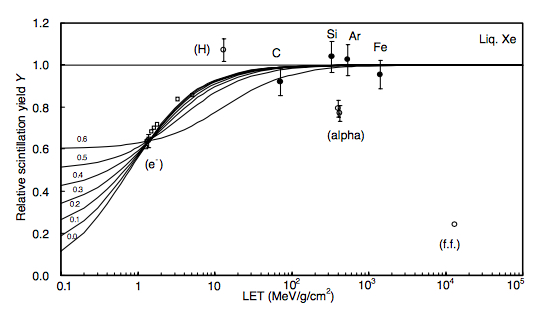
\includegraphics[width=0.8\textwidth]{ScintillationYield}
\caption{Scintillation yield as a function of LET in LXe.  Open circle represent electrons, alpha particles, and fission fragments.  Solid
circles represent relativistic heavy particles.  Open squares represent gamma-ray.  Solid lines represent various fits to the
$\beta$-$\gamma$
data performed in \citeref{Doke2002} and are not discussed here.  Image credit: \citeref{Doke2002}.}
\label{fig:scintillation_yield}
\end{figure}



%====================================
\section{Interactions}
\label{sec:interactions}
Because WIMP searches usually expect an interaction with an atom's nucleus, electronic recoils are not investigated for possible
signal.  Instead they play two major roles - the first is for calibrating the detector.  For larger detectors external sources are
not efficient since the the self-shielding of Xe makes it nearly impossible for radiation to penetrate the interior.  Thus internal
sources with short half-lifes such as \kryptonmeta and \radoncal are used.  The second role ER play is background to the DM
search.  Detector materials have radioactive elements that decay inside the detector, and long-lived intrinsic sources such as
the inevitable residual \krypton and \radon that passed the Xe distillation process.  The latter is much more concerning as events from
detectors materials cannot breach the fiducial volume, but intrinsic sources are uniformly distributed and must be understood.

\subsection{Photons}
\label{subsec:photons}
Photons produce electron recoils as they interact with \electron via Compton scattering pair production, or photoelectric absorption
as shown in \figref{fig:phot_atten}.  In Compton scattering the photon
recoils off of an \electron, transferring a portion of its energy.  Nuclear Compton scattering is possible but much rarer.  If the
angle of the scatter is known the change in energy can be determined.

Pair production is when a high-energy photon produces a particle-antiparticle pair.  Typically this refers to a photon passing sufficiently
near to an atom's nucleus creating an electron-positon pair.  The proximity of the nucleus is required to conserve momentum so it
recoils slightly as well.  The photon must have an energy of at least twice the mass of the electron $m_{e}$, or 1.022 MeV.  Pair production
also occurs for a photon in the presence of an atomic electron but is less probable and requires an energy of at least $4m_{e}$.  This
is known as triplet production since the recoiling electron will create a track in addition to the electron-positon pair
(\citeref{Hubbell2006}).  At high energies pair production becomes the dominant interaction for photons and matter.

Photoelectric absorption is when an electron absorbs the energy of the photon and is freed from its electron shell.  In this case the
photon disappears entirely and the kinetic energy of the electron is equal to the photon's energy minus the electron binding energy.  This
is a useful tool for calibrating small detectors with mono-energetic \gammarays from elements such as \cesium (661.7 keV) and \cobaltsixty
(1.1732 and 1.3325 MeV).  For larger detectors however the self-shielding prevents even the higher \gammarays from reaching the fiducial
volume, so external sources cannot be used for calibration.  Photoelectric absorption is the dominant interaction in the WIMP detection
energy region of interest, as shown in \figref{fig:phot_atten}.

\begin{figure}
 \centering
 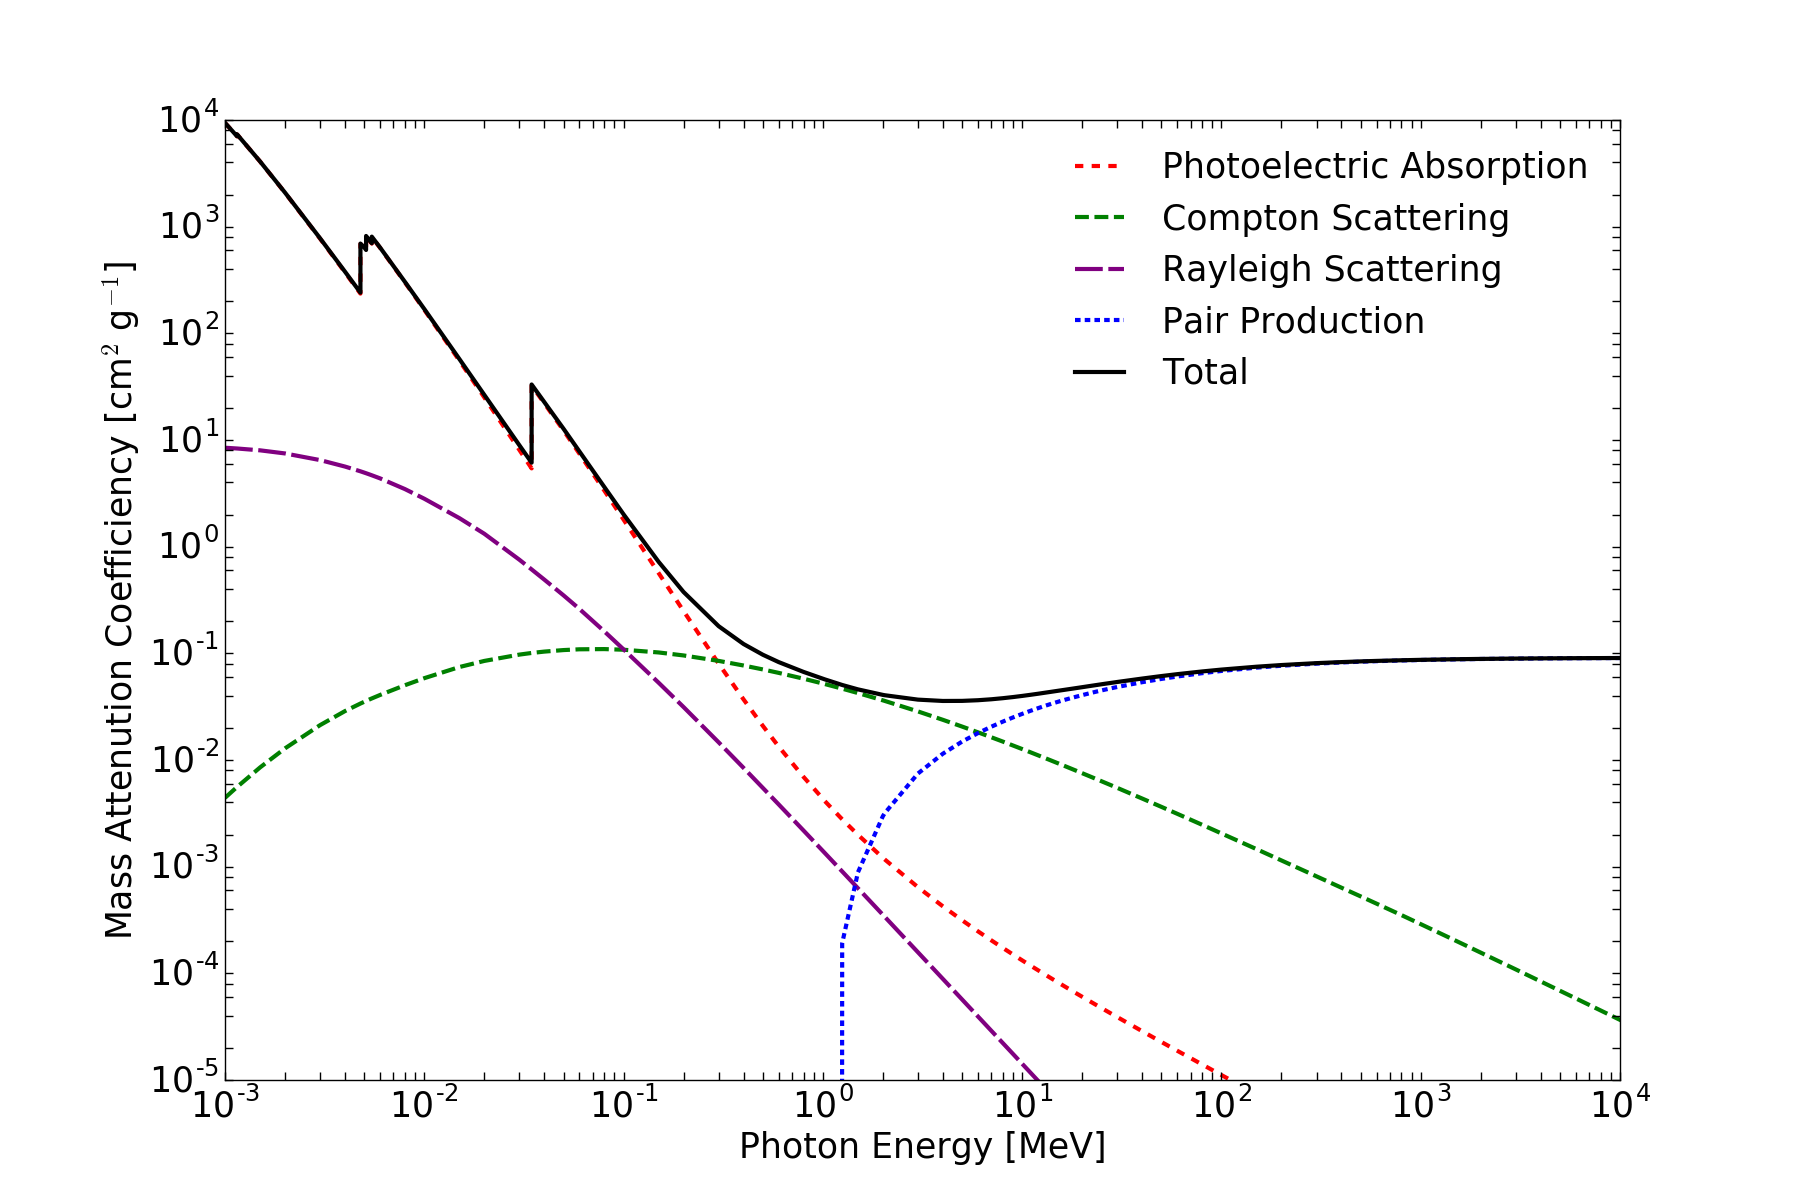
\includegraphics[width=0.8\textwidth]{PhotonAttenuation}
 \caption{Mass attenuation coefficient for photon energies $10^{-3} - 10^{4} \mathrm{MeV}$.  In addition to the total, values for
 photoelectric absorption,
 Compton scattering, and pair production are shown}
 \label{fig:phot_atten}
\end{figure}


\subsection{$\beta$-Decays}
\label{subsec:beta}
\betadecays are the emission of an electron-antineutrino (positron-neutrino) from a neutron (proton).  As with photons, they interact
with the \electron shell and thereby produce electronic recoils.  Because the neutrino carries
some momentum, the energy spectrum of the \electron is not mono-energetic, which makes it harder to identify the origin.  In Xe
experiments \betadecays contribute the most contamination in the search region for this reason and that they occur roughly uniformly
throughout the detector.  \krypton decays via

\begin{equation}
\ce{^{85}Kr} \rightarrow \ce{^{85}Rb} + e^{-} + \overline{\nu_{e}}
\end{equation}

\noindent with an energy of 687 keV with 99.53\% and 173 keV followed by a 514 $\gamma$ with 0.47\%.  These low-energy \betadecays
contaminate the search region, and a half-life of 10.72 years ensures \ce{^{85}Kr} will be present throughout the lifetime of the
experiment.

\ce{^{222}Rn} presents a similar problem.  As a daughter of the \ce{^{238}U} decay chain it emanates from the detector materials and
distributes
uniformly throughout the detector.  Its two most dangerous daughters or \leadtwofourteen and \ce{^{214}Bi}, each of which
undergo $\beta$-decay.  \ce{^{214}Bi} is easily identifiable because its daughter \poloniumtwofourteen has a half-life of
$160\ \mathrm{\mu s}$ and undergoes $\alpha$-decay.  Thus a cut on coincidence can remove such events.  \leadtwofourteen is more
dangerous, as it has no coincidence cut with its parent or daughter.  Its end-point energy when it decays to the ground state of
\bismuthtwofourteen is 1019 keV, which contaminates the region of interest.  More concerning is a decay to higher energy levels, which
if near the border of the fiducial volume has a risk of the subsequent \gammaray exiting undetected.  In XENON100 recoiling daughters of
the \ce{^{222}Rn} decay chain were observed to drift towards the cathode, possibly the result of becoming positively ionized
(\citeref{Weber2013}), lowering the number of \betadecays in the region of interest.


\subsection{Neutrinos}
\label{subsec:neutrinos}
Neutrinos impact both electronic and nuclear recoil spectra at low energies.  Solar neutrinos can elastically scatter off \electron
producing an ER.  \textit{pp} neutrinos make up 92\% of these scatters, with \ce{^{7}Be} making 7\%, and all other sources contributing
$<1$\% (\citeref{Aprile2016}).

Coherent neutrino-nucleus scattering produces nuclear recoils.  The majority of the interactions in the ROI come from Solar \ce{^{8}Be}
and \textit{hep} neutrinos, as those at higher energy from sources such as diffuse supernovae and the atmosphere have a significantly
lower rate.

Neutrinos are an irreducible background that affects our detector uniformly.


\subsection{Neutrons}
\label{subsec:neutrons}
Neutrons in our detector come from two main sources: the spontaneous fission (mainly $\alpha$) of isotopes of primordial chains of
\uranium, \ce{^{235}U}, and \ce{^{232}Th} from detector materials (radiogenic neutrons), and muons
passing through the rock and material above and around the detector (cosmogenic neutrons).  The former has energies in the MeV range
while the latter can reach tens of GeV (\citeref{Aprile2016}).  Neutrons have a mean free path on the order of tens of cm, which makes
them more difficult to shield than $\alpha$, $\beta$, or $\gamma$ scatters.  Furthermore, neutrons can produce nuclear recoils, making
them indistinguishable from WIMPs.  It is critical then to have a thorough understanding of the neutron background so a reliable
estimate of the number of events in the signal region to avoid mistaking a neutron as a WIMP or vice versa.

Neutrons will scatter elastically, inelastically, or be radiatively absorbed by the Xe nucleus.  Radiative absorption is when the
Xe nucleus captures the neutron, extending its atomic mass by one.  Fortunately, such an increase typically leads to another stable
xenon atom.  Exceptions are \ce{^{125}Xe}, \ce{^{127}Xe}, \ce{^{133}Xe}, and \ce{^{135}Xe}, which are listed in \tabref{tab:ncaption_xe}
along with subsequent decays and half-lives.  \ce{^{125}I} and \ce{^{135}Cs} have sufficiently long half-lives that they will be removed
by the getters from the LXe before they decay along with stable daughters \ce{^{127}I} and \ce{^{133}Cs}.

\bgroup
\def\arraystretch{1.4}
\begin{table}
 \centering
 \begin{tabular}{cccc}
 \centering
 Isotope & Decay & Energy [keV] & Half-Life \\
 \hline
 \ce{^{125}Xe} & $\ce{^{125}Xe} \rightarrow \ce{^{125}I} + \beta^{+} + \nu_{e}$ & 622.17 & 16.89 h \\
  & $\ce{^{125}I} + e^{-} \rightarrow \ce{^{125}Te} + \nu_{e}$ & 185.77 & 59.38 d \\
 \ce{^{127}Xe} & $\ce{^{127}Xe} + e^{-} \rightarrow \ce{^{127}I} + \nu_{e}$ & 662.33 & 36.34 d \\
 \ce{^{133}Xe} & $\ce{^{133}Xe} \rightarrow \ce{^{133}Cs} + \beta^{-} + \overline{\nu_{e}}$ & 427.36 & 5.24 d \\
 \ce{^{135}Xe} & $\ce{^{135}Xe} \rightarrow \ce{^{135}Cs} + \beta^{-} + \overline{\nu_{e}}$ & 1164.8 & 9.14 h \\
  & $\ce{^{135}Cs} \rightarrow \ce{^{135}Ba} + \beta^{-} + \overline{\nu_{e}}$ & 268.66 & $2.315 \times 10^{6}\ \mathrm{y}$ \\
 \hline
 \end{tabular}
 \caption{Radioactive isotopes of Xe produced from neutron capture.  Decays are shown to stable elements along with decay energies and
 half-lives}
 \label{tab:ncaption_xe}
\end{table}
\egroup

Inelastic scattering involves the neutron exciting the Xe nucleus.  It will still recoil from a nuclear interaction, but the Xe
activation follows with emission of a $\gamma$-ray.  The most relevant isotopes for our detector are \ce{^{129}Xe} and \ce{^{131}Xe},
which have half-lives of 0.97 and 0.48 ns and decay with energies 36.9 and 80.2 keV, respectively.  These lifetimes are much shorter
than the temporal resolution of the detector ($\mathcal{O}(10)\ \mathrm{ns}$) so the recoil and de-excitation will appear as a single
event.  However, the mean free path for the de-excitation photon is $\mathcal{O}(1)\ \mathrm{mm}$ so they may be spatially
resolvable (\citeref{McCabe2016}).  Additionally longer-lived activations for metastable
states $\ce{^{129\mathrm{m}}Xe}$ and $\ce{^{131\mathrm{m}}Xe}$ decay with with half-lives 8.88 and 11.93 days and energies 236.14 and 163.93 keV.  The
longer lifetimes allow the metastable xenon to become distributed uniformly throughout the detector, providing an internal calibration
over a period of weeks, which can be taken during dark matter data taking.  Inelastic scattering searches spin-dependent WIMPs so it
suffers in that it does not go with the square of the nucleon number as does spin-independent.

\begin{figure}
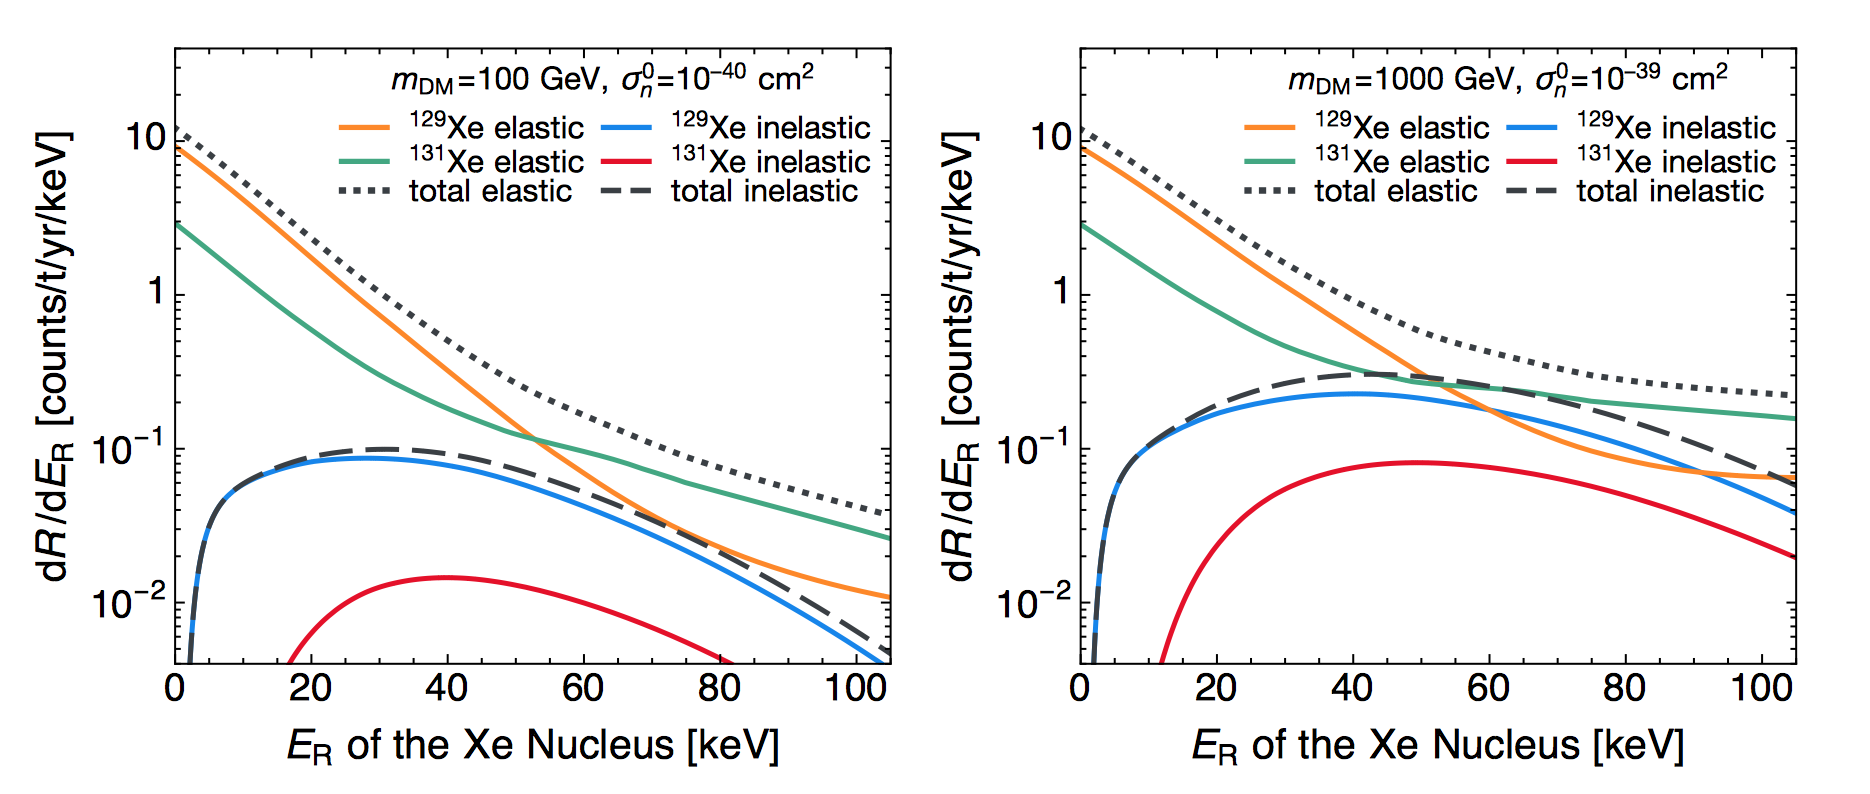
\includegraphics[width=\textwidth]{ElasticInelasticRates}
\caption{WIMP scattering rates for \ce{^{129}Xe} and \ce{^{131}Xe} for elastic and inelastic scatters.  Here the dark matter mass
$m_{\mathrm{DM}} \equiv m_{\chi}$ values are 100 GeV at a cross section of $\sigma_{n}^{0} = 10^{-40}\ \mathrm{cm^{2}}$ and
1000 GeV at a cross section of $\sigma_{n}^{0} = 10^{-39}\ \mathrm{cm^{2}}$. We see that elastic scattering is preferred across all
$E_{R}$, though at larger values inelastic has much more relative impact.  Furthermore the difference between the two is less in the
$m_{\mathrm{DM}} = 1000\ \mathrm{GeV}$ case, demonstrating that at higher $m_{\mathrm{DM}}$ the two become more comparable.  Inelastic
scattering drops to 0 at 
$E_{R} = 0\ \mathrm{keV}$ because conservation of momentum mandates the nucleus cannot be excited while the atom remains at rest
after an interaction.Figure credit: \citeref{McCabe2016}.}
\label{fig:nr_elastic_inelastic}
\end{figure}

The final interaction type is elastic scattering.  In this scenario the neutron rebounds from the nucleus and kinetic energy after the
scatter is preserved and distributed between the neutron and recoiling Xe atom.  Elastic scatters probe both spin-independence
and spin-dependence.  \figref{fig:nr_elastic_inelastic} shows the expected counts for \ce{^{129}Xe} and \ce{^{131}Xe} elastic and
inelastic scatterings for WIMPs of $m_{\chi} = 100,\ 1000\ \mathrm{GeV}$ with cross-sections of
$\sigma_{n}^{0} = 10^{-40},\ 10^{-39}\ \mathrm{cm^{2}}$.  We see that elastic scattering is dominant over inelastic, but at higher recoil
energies $E_{R}$ and larger WIMP masses the gap of the discrepancy decreases.  Elastic scattering is discussed further in
\secref{sec:nr} and \chapref{}.


%====================================
\section{Electronic Recoils}
\label{sec:er}
An electronic recoil signifies that the interaction occurred with the electron shell of an atom and the particle.  Because no energy
is lost to atomic motion the number of quanta produced is

\begin{equation}
N_{q} = \frac{E_{\mathrm{ER}}}{W}
\label{eq:nquant_er}
\end{equation}

\noindent where \energyer is the electronic recoil energy
and $W = 13.2\ \mathrm{eV}$ (\citeref{Dahl2009}) is the energy needed to produce a single quanta.  This can be broken up into

\begin{equation}
N_{q} = N_{\mathrm{ex}} + N_{\mathrm{i}}
\label{eq:quanta}
\end{equation}

\noindent where \nex and \nion is the number of excitons and ions, respectively.  The number of electron-ion pairs when a particle
deposits all of its energy has a root mean square of

\begin{equation}
\delta = F \times N_{\mathrm{i}}
\label{eq:fano}
\end{equation}

\noindent where $F < 1$ and known as the Fano factor (\citeref{Fano1947}).  Thus the fluctuations of $N_{\mathrm{i}}$ are smaller than a
Poisson
distribution ($F = 1$).  Several experiments have attempted to measure $F$ for LXe (\citeref{Doke1976, Seguinot1995}) with an
estimated value of $F = 0.056$ for \electron and $\gamma$-rays.  This places a limit on the fundamental energy resolution of

\begin{equation}
\Delta E = \sqrt{F W E}
\end{equation}

\noindent where $\Delta E$ is in keV, $W$ is in eV, and the energy $E$ is in MeV (\citeref{Aprile2009}).  Current LXe experiments have
not yet even achieved Poisson resolution, so there is a lot of progress that can be made in the future.

Rearranging \eqref{eq:quanta} we find the probability that a particular quanta is an ion

\begin{equation}
p_{\mathrm{ion}} = \frac{1}{1 + \frac{ N_{\mathrm{ex}} }{ N_{\mathrm{ion}} }}
\end{equation}

\noindent with $p_{\mathrm{ex}} = 1 - p_{\mathrm{ion}}$.  The ratio $N_{\mathrm{ex}} / N_{\mathrm{ion}}$ has been calculated to be
0.06 (\citeref{Takahashi1975})
but measurements today disagree (\citeref{Doke2002, Aprile2007}).  Currently $N_{\mathrm{ex}} / N_{\mathrm{ion}}$ is taken to be between
0.13-0.2.  The number of
photons and electrons after recombination can be found as

\begin{equation}
N_{\mathrm{phot}} = N_{\mathrm{ex}} + rN_{\mathrm{i}} \\
N_{\mathrm{e}} = (1 - r)N_{\mathrm{i}}
\end{equation}

\noindent where \nphot is the number of photons produced and \nelect is the number of \electron that do not recombine and are extracted as
proportional scintillation.

Although noble gas detectors allow ER-NR discrimination, the two regions are near one another and have overlap where an event could
be considered with reasonable probability to be either.  In the DM search only the region of NR-space where the NR likelihood is
significantly more probable is used.  To minimize the risk of ER, or background events from occurring in the signal region it is
critical to reduce the background as much as possible, and with the ton-scale era of DM detectors underway much effort is being put into
material screening and enhanced xenon distillation.


%====================================
\section{Nuclear Recoils}
\label{sec:nr}
Although the vast majority of background comes from electronic recoils, nuclear recoils are more dangerous because they replicate
WIMP interactions.  Therefore the NR background must be well-modeled to avoid mistaking a background event for a WIMP or vice
versa.

\noindent Atomic motion in liquid noble gas experiments is not observable any energy that is passed on as kinetic energy to the nucleus
is lost.  While energized electrons are capable of transferring very small
amounts of energy to the motion of the nucleus, the reverse is not true.  Atomic motion has only been observed in nuclear recoils,
which implies for the same energy deposition $N_{q}$ will differ between electronic and nuclear recoils.  The fraction of energy lost
to atomic motion is characterized by $f_{n}$, which is commonly characterized by the Lindhard model
(\citeref{Lindhard1965})

\begin{equation}
f_{n} = \frac{k g(\epsilon)}{1 + k g(\epsilon)}
\label{eq:linhard_quenching}
\end{equation}

\noindent where $k = 0.133Z^{2/3}A^{1/2}$, $g(\epsilon) = 3\epsilon^{0.15} + 0.7\epsilon^{0.6} + \epsilon$, and
$\epsilon = 11.5 (E_{R} / Z^{7/3})$ where $Z$ is the atomic number and $A$ is the number of nucleons.  $k$ is proportional to the ratio of
electronic stopping power to particle velocity of the recoiling Xe atom (\citeref{Sorensen2011}) and $g(\epsilon)$ is proportional
to the ratio of electronic to nuclear scaling factor (\citeref{NEST2015}).  There has been some debate about
the coefficient in $k$ and I use the value from \citeref{Lewin1996}.  Studies have shown that energy is only lost to atomic motion for
nuclear recoils.  When parameterized by the Lindhard model the quenching factor $f_{n}$ is sometimes written as $L(E)$.  It is
shown in \figref{fig:lindhard} for the relevant energy search region.

\begin{figure}
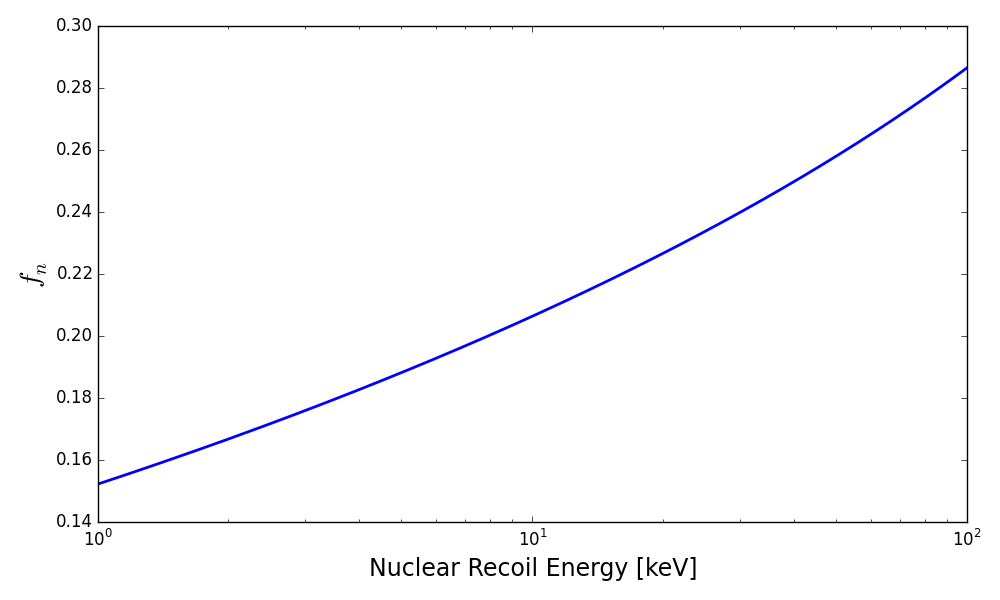
\includegraphics[width=0.8\textwidth]{Lindhard}
\caption{Fraction of nuclear energy passed to atomic motion in xenon using Lindhard's theory (\citeref{Lindhard1965}).}
\label{fig:lindhard}
\end{figure}

In addition primary scintillation is subject to biexcitonic quenching and reduced by a factor of $1 - f_{l}$.  The total number of quanta
is

\begin{equation}
N_{q} = \frac{L(E) E_{\mathrm{NR}}}{W}
\label{eq:nquant_nr}
\end{equation}

\noindent Note the difference between \eqref{eq:nquant_er} and \eqref{eq:nquant_nr} is simply $L(E)$ as well as the the recoil energy
scale (discussed in \secref{}).  Unlike ERs, $N_{\mathrm{ex}} / N_{\mathrm{i}} \sim 1$ (\citeref{Sorensen2011, Angle2011}) due to the
higher density tracks.



%====================================
\section{Time Projection Chambers}
\label{sec:tpcs}
Time projection chambers (TPCs) measures the light and charge of an interaction in the noble liquid.  They have been leading the
spin-independent search for WIMP masses $> 10\ \mathrm{GeV}$ and as the ton-scale era progresses are poised to continue.  In this section
only liquid noble gases TPCs relevant for dark matter searches are discussed.

\subsection{Working Principle}
\label{subsec:tpcs_working_principle}
TPCs consist of a liquid noble element with a small gas gap at the top.  At least three meshes are required for a functioning TPC: the
cathode, gate, and anode, all of which are parallel.  A diagram of a TPC with an event is shown in \figref{fig:tpcs_tpc}.  The cathode is
at the bottom of the detector and applies an electric field - known as the drift field $E_{d}$ - between
it and the gate, which is grounded.  The liquid level is set to just above the gate.  As briefly covered in \secref{subsec:secondary}
$E_{d}$ will push any \electron that do not recombine towards the surface of the liquid at drift velocity $v_{d}$.  Typically an electric
field cage consisting
of metal rings stacked vertically, or parallel to the cathode and gate.  They are connected via resistors such that they mirror the
the drift field, helping to maintain field uniformity.

\begin{figure}
\includegraphics[width=\textwidth]{}
\label{fig:tpcs_tpc}
\end{figure}

The body of \electron that move along $E_{d}$ are known as the electron cloud.  As the electron cloud drifts it diffuses both
longitudinally (in the direction of $E_{d}$) and transversely (perpendicular to $E_{d}$).  The
diffusion coefficients $D_{L}$ and $D_{T}$ are dependent on the electric field with $D_{T}/D_{L} \sim 10$.  The electron spread can
be written as $\sigma_{D_{T}} = \sqrt{D_{T} t_{d}}$ where $t_{d} = d/v_{d}$ is the drift time and $d$ is the drift distance.

While xenon distillation inevitably leaves residual noble gases, it is much more effective at removing other elements.  Nonetheless
impurities that outgas from detector materials contaminate the noble gas.  Electronegative impurities in particular present a problem
since they attach to drifting $e^{-1}$,
lowering the number that reach the liquid-gas interface and thus decreasing the secondary scintillation.  The attachment process
is
\eqref{eq:impurity_attach}.

\begin{equation}
e^{-} + S \rightarrow S^{-}
\label{eq:impurity_attach}
\end{equation}

\noindent where $S$ is the impurity.  The number of \electron captured is dependent drift time $t_{d}$ and the
attachment rate of
the impurities $k_{S}$, both of which depend on $E_{d}$.  Clearly then an advantage of larger
\efields is a larger
\vd (up to a point, see \figref{fig:drift_velocity}) and thus less time in the liquid.  Doping LXe with organic materials such as butane
can increase \vd at stronger
\efields but are not used in DM detectors due to difficulty in purifying (\citeref{Yoshino1976}).  The rate at which electrons are
absorbed by impurities is proportional to the number of electrons, impurities, and impurity attachment rate.  Assuming the the density
of impurities in the liquid and $E_{d}$ are uniform we find

\begin{equation}
\frac{dq}{dt} = -qk_{S}S
\label{eq:lifetime_diff_eq}
\end{equation}

\begin{equation}
q(t) = q_{0}e^{-tk_{S}S} = q_{0}e^{-t/\tau_{e}}
\label{eq:lifetime_equation}
\end{equation}

\noindent where $\tau_{e} = (k_{S}S)^{-1}$ is the electron lifetime.  $k_{S}$ is shown in \figref{fig:attachment_rate} for
O$_{2}$,
N$_{2}$O, and SF$_{6}$.  We see that for N$_{2}$O the attaching rate constant increases with \efield whereas \otwo and SF$_{6}$
decerase.  Typically impurity concentration is given in O$_{2}$-equivalent values, or the concentration of \otwo if it was solely
responsible for \electron attachment.  For modeling electron lifetime it turns out that using the \otwo curve in
\figref{fig:attachment_rate} gives a good approximation as it is expected to the most dominant (\textbf{check this}).  Removing these
impurities
will be discussed in detail in \secref{}.

\begin{figure}
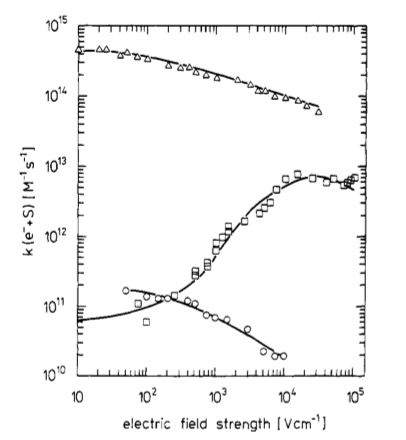
\includegraphics[width=0.8\textwidth]{AttachmentRate}
\caption{Attaching rate constant $k_{S}$ from \citeref{Bakale1976} for \otwo, N$_{2}$O, and SF$_{6}$ with respect to electric field.  At
larger \efield $k_{S}$ increases for N$_{2}$O and decreases for \otwo and SF$_{6}$.}
\label{fig:attachment_rate}
\end{figure}

About a centimeter (\textbf{check this}) above the gate is the anode.  The electric field between the gate and anode $E_{g}$ must be strong
enough to extract the \electron that reach the liquid surface into the gas.  To do this the anode is typically set to
$V_{a} \sim 4000\ \mathrm{kV\ cm^{-1}}$.  An extracted \electron will quickly gain enough kinetic energy to ionize atoms in the gas,
whose \electron in turn ionize others, creating a cascade effect.  Because the scintillation per electron is independent of
the total number of electrons extracted this is known as proportional scintillation.  It is also known as secondary scintillation or
electroluminescence.  The number of photons $N_{\mathrm{ph}}$ produced over a distance $z$ per \electron is

\begin{equation}
\frac{dN_{\mathrm{ph}}}{dz} = \alpha \Big( \frac{E_{g}}{P} - \beta \Big) P
\label{eq:electronlum}
\end{equation}

\noindent where $\alpha = 70\ \mathrm{photons\ kV^{-1}}$, $\beta = 1.0\ \mathrm{kV\ cm^{-1}\ atm^{-1}}$, and $P$ is the pressure in the
gas (\citeref{Belogurov1995}).

TPCs have photodetectors at the top (above the gate) and bottom (below the cathode).  While proportional scintillation occurs at the top
and in most detector settings produces enough light to guarantee detection, prompt scintillation - especially for low energy events - does
not have this benefit.  Depending on the geometry of the detector the fraction of light that is directed towards the photodetectors can
be small, and the photodetectors themselves can have less than unity photon detection efficiency (\secref{subsec:tpcs_pmts}).  PMTs cannot
be fixed around the cylindrical portion of the TPC because it would interfere with the drift field created by the field cage.  To increase
the intensity of light that reaches the photodetectors, and thereby improve the likelihood that an event is
detected, the wall of the TPC is covered in a reflective material just inside the field cage.  Polytetrafluoroethylene (PTFE) is
reflective for liquid noble gas scintillation (in the UV range) and is a common choice.  It has been shown to have $> 97 \%$
reflectance when immersed in LXe to 178 nm, the xenon scintillation wavelength (\citeref{Neves2017}).


\subsection{Photomultiplier Tubes}
\label{subsec:tpcs_pmts}
Photomultiplier tubes (PMTs) are used for light detection in TPCs.  A digram of a PMT is shown in \figref{fig:tpcs_pmts_pmt_diagram}.  An
incoming photon that
passes through the window of the PMT will most often hit the photocathode, freeing a photoelectron via the photoelectric effect.  Single
photoelectron emission (SPE) refers to a photon freeing a single \electron from the photocathode.  The
quantum efficiency (QE), which is the ratio of electrons ejected from the photocathode divided by incident photons, is approximately
one third.  Because of this relatively low value choosing a highly reflective material for the TPC wall is critical.  The QE spectrum for
the PMTs used in XENON1T, Hamamatsu R11410, is shown in \figref{fig:tpcs_pmts_qe}.  Note the maximum is near 178 nm, making it a good
choice for LXe TPCs.  Once ejected, the photoelectron passes through the focusing
electrode, which directs it towards the first dynode.  The dynodes are coupled to one another through resistors, lowering the electric
potential with each successive one.  As the photoelectron hits the first dynode it will free electrons.  These will then pass to the
second dynode, repeating this procedure.  This results in a cascade effect ending at the anode, where the charge is output to a
voltage reading device such as an oscilloscope or digitizer.

\begin{figure}
\centering
\includegraphics[width=0.6\textwidth]{Fig4FromLung2012}
\caption{Quantum efficiency with respect to wavelength for the Hamamatsu R11410 PMT, used in XENON1T.  The peak efficiency occurs near
the xenon scintillation wavelength 178 nm at $\sim 35 \%$.  The sharp cutoff to the left is due to the quartz window.  Image credit:
\citeref{Lung2012}.}
\label{fig:tpcs_pmts_qe}
\end{figure}

In some cases an incident photon may pass through the photocathode and directly hit the first dynode, freeing an electron.  This will
cause the same response as a photocathode ionization except with one fewer dynode, leading to an under-amplified current.  Additionally,
if the incident photon has at least double the workfunction of the photocathode we would expect the number of photoelectrons emitted to
follow a Poisson distribution.  However, a recent study of several Hamamatsu vacuum ultraviolet-sensitive (VUV) PMTs showed the double
photoelectron emission
(DPE) fraction was between 18-24\% depending on the PMT, higher than the expected $\sim 15\%$.  This includes the PMTs that are used in
XENON100 and XENON1T.

\begin{figure}
\centering
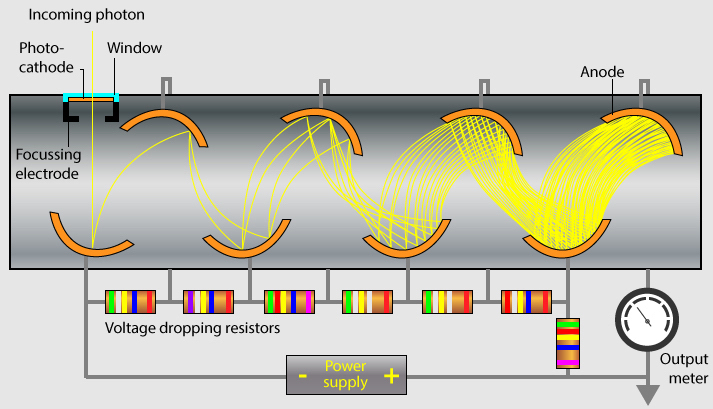
\includegraphics[width=\textwidth]{PMT1}
\caption{Diagram of a PMT.  An incident photon hits the photocathode, freeing a photoelectron.  With each dynode the more \electron are
freed, creating an amplified signal that is eventually output.  Image credit: \citeref{CHROMacademy}.}
\label{fig:tpcs_pmts_pmt_diagram}
\end{figure}

Afterpulses are an increase in PMT signal directly following and as a consequence of the true signal.  Afterpulses precipitate from one of
two categories.  The first is the elastic scattering of \electron with the initial dynode, prompting afterpulses in the range of a few
to tens of nanoseconds.  The second is triggered by positive ions of residual gases in the body of the PMT striking the photocathode,
expelling additional photoelectrons.  The number of photoelectrons (amplitude of afterpulse) depends on the ion and position of
ionization.  The delay between true signal and afterpulse of this class is between hundreds of nanoseconds and several microseconds,
depending on the ion and voltage of the PMT.  Afterpulse amplitude vs. delay time can be seen in \figref{fig:tpcs_pmts_ap}.  Afterpulses
constitute a problem because, depending on the delay and magnitude of the true
signal, can be difficult to distinguish from the actual signal.  The extent of afterpulses from the second classification is directly
related to the number of residual gas in the PMT.  Thus achieving excellent vacuum is a necessity - indeed, too much residual gas will
lead to deterioration of and ultimately inability to operate the PMT.

\begin{figure}
\centering
\includegraphics[width=\textwidth]{Afterpulse}
\caption{Afterpulses for one of the PMTs from XENON1T.}
\label{fig:tpcs_pmts_ap}
\end{figure}

Liquid noble gases used in dark matter searches emit ultraviolet light.  Scintillation is at 178 nm for xenon, 128 nm for argon, and
78 nm for neon.  LAr experiments have to use wavelength shifters because current PMTs are not sensitive to such low wavelengths.  For
LXe this is not a problem as PMTs have good sensitivity to 178 nm.  Details of the PMTs used in XENON1T can be found in \secref{}.



\subsection{Signals}
\label{subsec:tpcs_signals}
Primary and secondary scintillation are measured in units of photoelectrons and denoted S1 and S2, respectively.  An example of an
interaction is shown in \figref{fig:tpcs_signal_tpc}.  In the left side a particle scatters with the LXe, prompting photons almost
immediately that are observed by the PMTs.  The right side shows the freed \electron that have drifted to the LXe-GXe interface and
are extracted by the anode across the GXe.  The PMTs are colored with relative intensity they would observe.  For a typical S1 the
bottom PMTs observed more light due to reflection off the LXe surface (though the amount depends on where in the TPC the interaction
occurs).  For S2s the top PMTs see more light since the amplification occurs close and directly underneath them.  Note that for S2s
the top PMTs have an intensity profile centered around where the \electron are extracted.  The bottom PMTs have a roughly uniform
distribution as the light has more area to separate, as well as reflect off the walls.

\begin{figure}
\centering
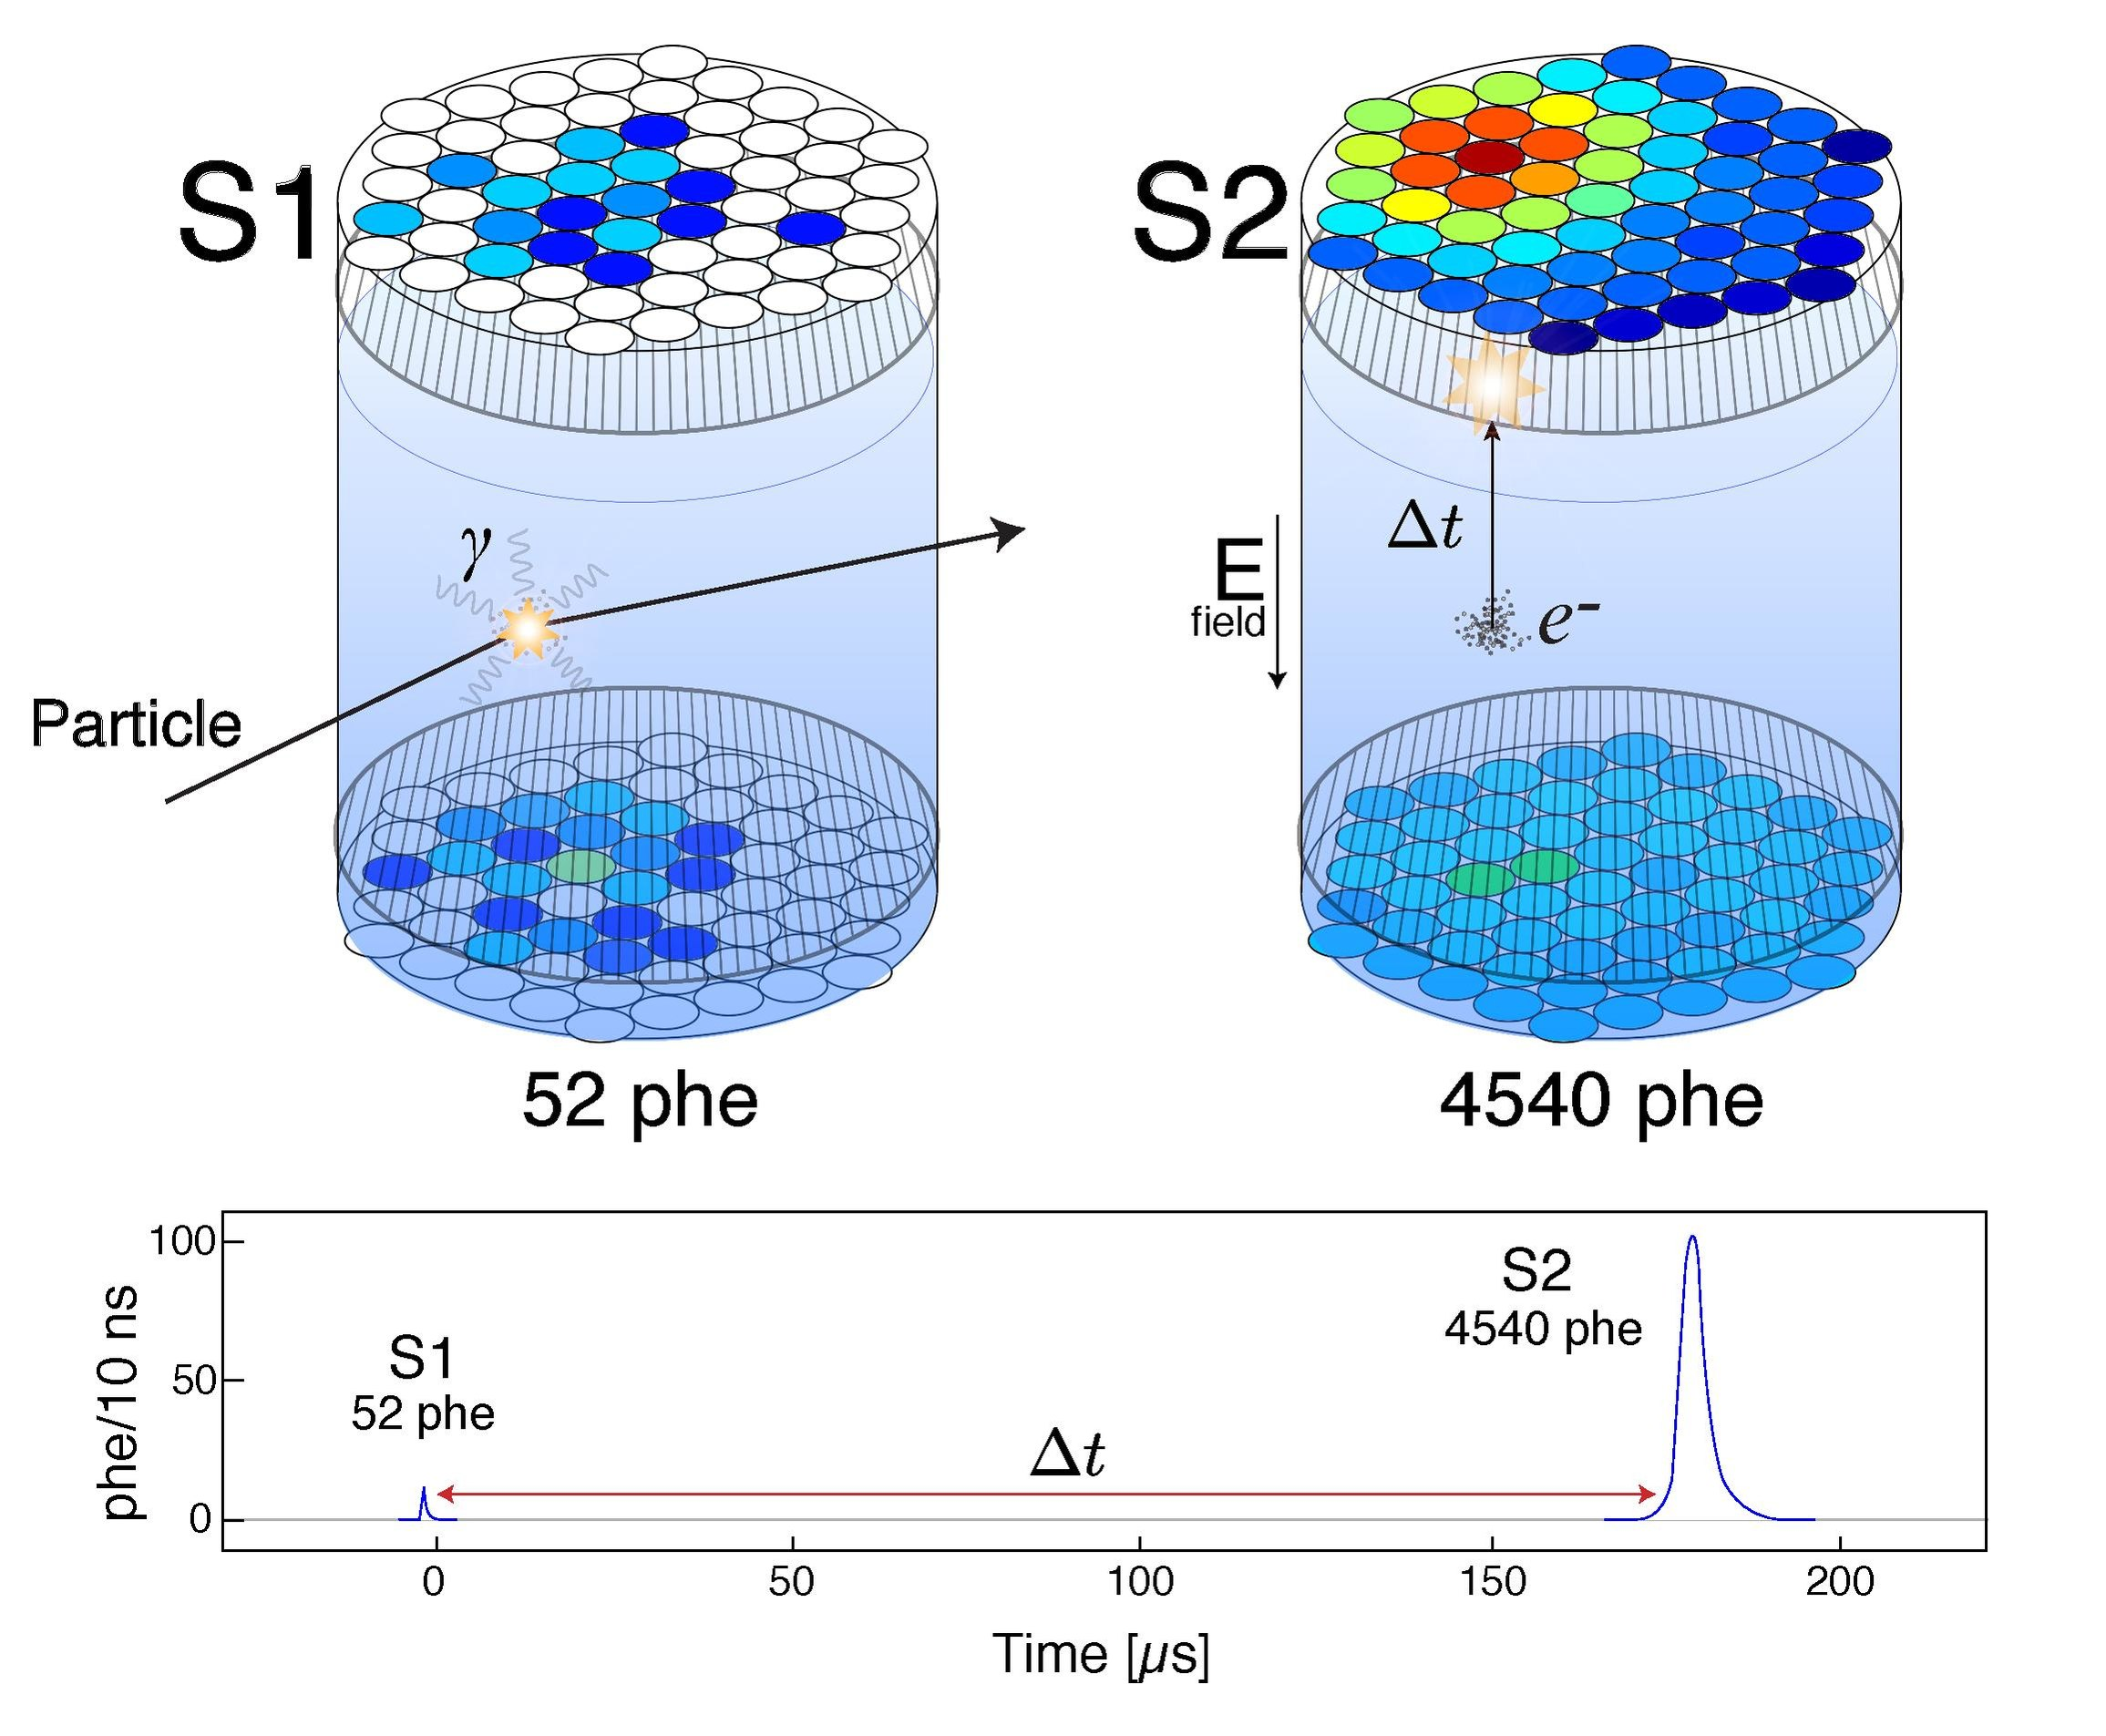
\includegraphics[width=\textwidth]{LUXTPC}
\caption{A diagram of an interaction in a LXe TPC.  The primary scintillation (S1) is immediately
observed by the PMT arrays.  The \electron drift under $E_{d}$ towards the top of the detector, where they are extracted across GXe,
creating secondary scintillation (S2).  The plot at the bottom depicts what a typical waveform looks like.  Note the S2 is significantly
higher than the S1 due to the amplification during electroluminescence.  The relative intensity of light in the PMTs, or PMT hit
pattern, can be used to determine the x- and y-coordinates of the interaction.}
\label{fig:tpcs_signal_tpc}
\end{figure}



\subsubsection{Position Reconstruction}
\label{subsubsec:tpcs_signals_posrec}
In addition to knowing the z-coordinate of the interaction ($\mathrm{z} = v_{d} t_{d}$) TPCs can recove the x and y positions.  The S2
hit pattern in the top PMT panel in \figref{fig:tpcs_signal_tpc} very clearly shows an intensity distribution that peaks at one
PMT and dissipates outwards.  It seems likely then that the S2 was extracted beneath or nearly beneath this PMT then.  A variety of
algorithms can be applied to PMT hit patterns to estimate the x-y position of the event.  Typically the resolution of event
reconstruction depends on the number and area of PMTs as well as the S2 size.  \figref{fig:tpcs_signals_posrec} shows the event
distribution for XENON1T Science Run 1.  The majority of events are near the wall, a consequence from the
traces of radioactivity present in detector materials.  The large self-shielding of LXe constrains nearly all of these to within
$\sim 5\ \mathrm{cm}$ of the wall, enabling a reasonably large fiducial volume.

\begin{figure}
    \centering
    \begin{subfigure}[t]{0.45\textwidth}
        \centering
        \includegraphics[height=4.5cm]{PosRecXY}
    \end{subfigure}%
    \begin{subfigure}[t]{0.45\textwidth}
        \centering
        \includegraphics[height=4.5cm]{PosRecRZ}
    \end{subfigure}
    \caption{Position reconstruction for events in XENON1T Science Run 1.  Top PMT hit patterns are used to determine x-y while
    $\mathrm{z} = v_{d} t_{d}$.  The number of events drops dramatically at lower radii due to the self-shielding of LXe.}
	\label{fig:tpcs_signals_posrec}
\end{figure}



\subsubsection{Discrimination}
\label{subsubsec:tpcs_signals_discr}
As discussed in \secref{subsec:stopping_power} the track structure affects recombination (\secref{subsec:recombination}), thereby
influencing the S1 and S2.  \figref{fig:mass_stopping_power} shows that the stopping power, and therefore track structure, changes
with energy for a given particle, so we expect S2/S1 to vary.  Because the track structure of a neutron is denser than $\beta$ and
$\gamma$ recombination should yield different prompt and proportional scintillations.  While we know nuclear recoils lose a
non-negligible fraction of energy to atomic motion
(\secref{sec:nr}), it is still possible to apply ER-NR discrimination by looking at S1-space instead.

\figref{fig:tpcs_signals_ernr} shows S2 vs. S1 for electronic and nuclear recoils.  The electronic are from a \ce{^{220}Rn} calibration
where the \ce{^{212}Pb} daughter undergoes $\beta^{-}$ decay.  The short lifetime of the \ce{^{220}Rn} decay chain, low energy
recoil (569.9 end-point energy), and uniform distribution throughout the detector make \ce{^{220}Rn} an excellent choice for
ER calibration.

Unfortunately there are no noble gas neutron sources
for calibrating inside the TPC and other elements would lower the purity of the detector, significantly decreasing the electron
lifetime.  Therefore nuclear calibrations must be done with external sources, limiting the number of events in the FV.  For XENON1T
these were done with americium beryllium (AmBe) and a neutron generator.  The nuclear recoils in \figref{fig:tpcs_signal_ernr} are from
an AmBe calibration during Science Run 1 with $E = ?\ \mathrm{kV\ cm^{-1}}$.

As expected from the less concentrated track structure we see that the \ce{^{220}Rn}
has on average larger S2s for a given S1, meaning that even though we are not comparing energies, the change in stopping
power between the ER and NR energies still results in a denser track for NR.  This holds true in general, giving

\begin{equation}
\Big( \frac{\mathrm{S}2}{\mathrm{S}1} \Big)_{\mathrm{ER}} > \Big( \frac{\mathrm{S}2}{\mathrm{S}1} \Big)_{\mathrm{NR}}
\end{equation}

for all S1s.

\begin{figure}
\centering
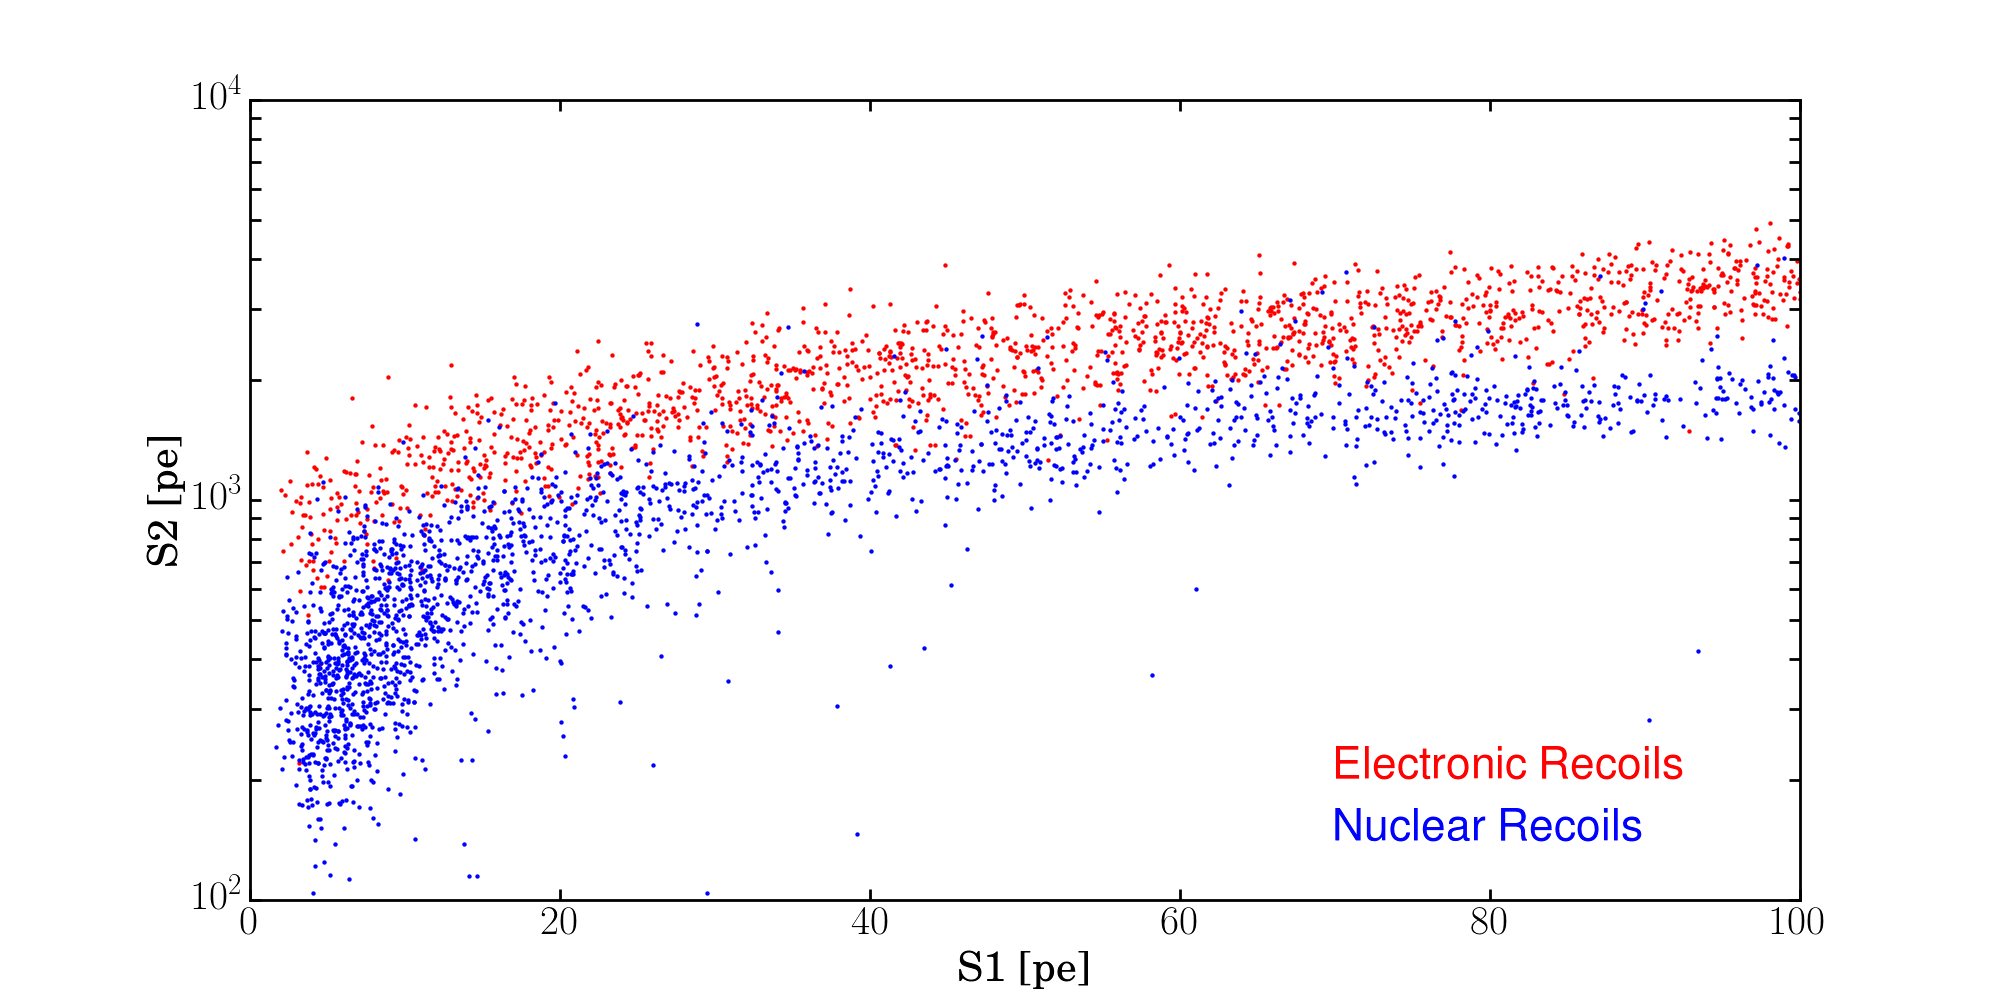
\includegraphics[width=\textwidth]{ERNRComparison}
\caption{S2 (proportional) vs. S1 (prompt) for recoils in LXe.  Electronic recoils are from the \ce{^{220}Rn} decay chain where
\ce{^{212}Pb} undergoes $\beta^{-}$ decay with an end-point energy of 569.9 keV (\textbf{check this}) and are shown in red.  Nuclear
recoils are from americium beryllium (AmBe) and are shown in blue.  We see the ratio of S2/S1 is larger for electronic recoils,
allowing discrimination between possible WIMPs and ER background.}
\label{fig:tpcs_signals_ernr}
\end{figure}

It is possible to reconstruct the number of photons and electrons from an S1 and S2.  Doing so requires knowing a number of detector
variables, including PMT quantum efficiency, light per extracted $e^{-1}$, light collection efficiency (LCE) variation throughout
the TPC, and more.  These are discussed in detail in \secref{}.  If these are well-understood the number of photons and electrons,
can be calculated.  Typically these are given in photoelectrons per photon and photoelectrons per \electron and are designated by
light and charge yield, respectively (details in \secref{}).  \figref{figs:tpcs_signals_drift_field} shows the ratios of light and
charge yield as a function of drift field for 122 keV electron recoils (\ce{^{57}Co} $\gamma$-rays), 56.5 keV elastic nuclear recoils, and
5.5 MeV $\alpha$-decays.  Expectedly at larger drift fields the light yield declines while the charge increases.  The sparser
ionization density directs electronic recoils to be significantly more influenced than nuclear or alphas.  This dissimilarity reveals
the drift field can be optimized for ER-NR discrimination.

\begin{figure}
\centering
\includegraphics[width=0.8\textwidth]{LightChargeYieldDriftField}
\caption{Ratio of light (S(E)/S$_{0}$, red) and charge (Q(E)/Q$_{0}$, blue) yields vs. drift field.  S$_{0}$ and Q$_{0}$ are taken at
infinite field.  Electronic recoils are shown as solid diamonds and are from the 122 keV \gammaray of \ce{^{57}Co}.  Nuclear recoils
are shown as empty squares and are from elastic 56.5 keV scatters.  Solid circles represent the 5.5 MeV $\alpha$-decay of
\ce{^{241}Am}.  Sparser ionization densities precipitate stronger field-dependence for electronic scatters than for nuclear and
alpha, signifying $E_{d}$ can be tuned for improved ER-NR discrimination.  Image credit: \citeref{Aprile2006}.}
\label{fig:tpcs_signals_drift_field}
\end{figure}



























% for stopping power look at A Model of Nuclear Recoil Scintillation Efficiency in Noble Liquids
%D.-M. Mei a,∗ Z.-B. Yin a,b,1, L.C. Stonehill c, A. Hime c


%Lewin and Smith (1996) - Lindhard factor
%Doke et al., 2002 - LET
%Miller et al., 1968 - drift velocity








% for kr/xe level
%E Aprile, J Aalbers, F Agostini, M Alfonsi, F. Amaro, M Anthony, F Arneodo, P Barrow, L Baudis, B. Bauermeister, et al., “Removing krypton from xenon by cryogenic distillation to the ppq level,” The European Physical Journal C, vol. 77, no. 5, p. 275, 2017.